\documentclass[main.tex,fontsize=8pt,paper=a4,paper=portrait,DIV=calc,]{scrartcl}
% Document
\usepackage[T1]{fontenc}
\usepackage[utf8]{inputenc}
\usepackage[dvipsnames]{xcolor}
\usepackage[nswissgerman,english]{babel} 
\usepackage{hyperref}
\renewcommand{\familydefault}{\sfdefault}

% Format
\usepackage[top=5mm,bottom=1mm,left=5mm,right=5mm]{geometry}
%\setlength{\headheight}{\baselineskip}
%\setlength{\headsep}{0mm}

%\usepackage{scrlayer-scrpage}
%\clearpairofpagestyles
%\chead{{\bfseries\TITLE, \AUTHOR, \pagename~\thepage}}

%\addtokomafont{pagehead}{\upshape}

\usepackage{multicol}
\setlength{\columnsep}{2mm}
\setlength{\columnseprule}{0.1pt}

% Math
\usepackage{amsmath}
\usepackage{amssymb}
\usepackage{amsfonts}

% Code
\usepackage{fancyvrb, etoolbox, listings, xcolor}
%\usemintedstyle{bw}

%\newminted[shell]{bash}{
%fontsize=\footnotesize,
%fontfamily=tt,
%breaklines=true,
%frame=single,
%framerule=0.1pt,
%framesep=2mm,
%tabsize=2
%}
%\newminted{css}{
%breaklines=true,
%tabsize=4,
%autogobble=true,
%escapeinside=||,
%stripall=true,
%stripnl=true,
%}

    \definecolor{lightgray}{rgb}{0.95, 0.95, 0.95}
    \definecolor{darkgray}{rgb}{0.4, 0.4, 0.4}
    \definecolor{purple}{rgb}{0.65, 0.12, 0.82}
    \definecolor{ocherCode}{rgb}{1, 0.5, 0} % #FF7F00 -> rgb(239, 169, 0)
    \definecolor{blueCode}{rgb}{0, 0, 0.93} % #0000EE -> rgb(0, 0, 238)
    \definecolor{greenCode}{rgb}{0, 0.6, 0} % #009900 -> rgb(0, 153, 0)
    \definecolor{teal}{rgb}{0.0, 0.5, 0.5}

\lstdefinestyle{code}{
    identifierstyle=\color{black},
    keywordstyle=\color{blue}\bfseries\small,
    ndkeywordstyle=\color{greenCode}\bfseries\small,
    stringstyle=\color{ocherCode}\ttfamily\small,
    commentstyle=\color{teal}\ttfamily\textit\small,
    basicstyle=\ttfamily\small,
    breakatwhitespace=false,         
    breaklines=true,                 
    captionpos=b,                    
    keepspaces=true,                 
    showspaces=false,                
    showstringspaces=false,
    showtabs=false,                  
    tabsize=2,
    belowskip=-5pt
}



% Images
\usepackage{graphicx}
\newcommand{\pic}{\includegraphics[scale=0.3]}
\graphicspath{{Screenshots/}{../Screenshots}}
\makeatletter
\def\pictext#1#2{%
    \@ifnextchar[{%
    \pictext@iiiii{#1}{#2}%
    }{%
      \pictext@iiiii{#1}{#2}[0.5,0.4,0.3]% Default is 5
    }%
}
\def\pictext@iiiii#1#2[#3,#4,#5]{\begin{minipage}{#3\textwidth}\includegraphics[scale=#4]{#1}\end{minipage}\begin{minipage}{#5\textwidth}#2\end{minipage}}
\def\minipg#1#2{%
    \@ifnextchar[{%
    \minipg@iiii{#1}{#2}%
    }{%
      \minipg@iiii{#1}{#2}[0.3,0.6]% Default is 5
    }%
}
\def\minipg@iiii#1#2[#3,#4]{\vspace{0.8mm}\begin{minipage}{#3\textwidth}#1\end{minipage}\begin{minipage}{#4\textwidth}#2\end{minipage}{\vspace{0.8mm}}}
\makeatother

%\newenvironment{minty}[2]% environment name
%{% begin code
%  \begin{minipage}{#1}
%  \begin{minted}{#2}
%}%
%{% end code
%  \end{minted}
%  \end{minipage}
%  \end{minty}\ignorespacesafterend
%} 

% Smaller Lists
\usepackage{enumitem}
\setlist[itemize,enumerate]{leftmargin=3mm, labelindent=0mm, labelwidth=1mm, labelsep=1mm, nosep}
\setlist[description]{leftmargin=0mm, nosep}
\setlength{\parindent}{0cm}

% Smaller Titles
\usepackage[explicit]{titlesec}

%% Color Boxes
\newcommand{\sectioncolor}[1]{\colorbox{black!60}{\parbox{0.989\linewidth}{\color{white}#1}}}
\newcommand{\subsectioncolor}[1]{\colorbox{black!50}{\parbox{0.989\linewidth}{\color{white}#1}}}
\newcommand{\subsubsectioncolor}[1]{\colorbox{black!40}{\parbox{0.989\linewidth}{\color{white}#1}}}
\newcommand{\paragraphcolor}[1]{\colorbox{black!30}{\parbox{0.989\linewidth}{\color{white}#1}}}
\newcommand{\subparagraphcolor}[1]{\colorbox{black!20}{\parbox{0.989\linewidth}{\color{white}#1}}}

%% Title Format
\titleformat{\section}{\vspace{0.5mm}\bfseries}{}{0mm}{\sectioncolor{\thesection~#1}}[{\vspace{0.5mm}}]
\titleformat{\subsection}{\vspace{0.5mm}\bfseries}{}{0mm}{\subsectioncolor{\thesubsection~#1}}[{\vspace{0.5mm}}]
\titleformat{\subsubsection}{\vspace{0.5mm}\bfseries}{}{0mm}{\subsubsectioncolor{\thesubsubsection~#1}}[{\vspace{0.5mm}}]
\titleformat{\paragraph}{\vspace{0.5mm}\bfseries}{}{0mm}{\paragraphcolor{\theparagraph~#1}}[{\vspace{0.5mm}}]
\titleformat{\subparagraph}{\vspace{0.5mm}\bfseries}{}{0mm}{\subparagraphcolor{\thesubparagraph~#1}}[{\vspace{0.5mm}}]

%% Title Spacing
\titlespacing{\section}{0mm}{0mm}{0mm}
\titlespacing{\subsection}{0mm}{0mm}{0mm}
\titlespacing{\subsubsection}{0mm}{0mm}{0mm}
\titlespacing{\paragraph}{0mm}{0mm}{0mm}
\titlespacing{\subparagraph}{0mm}{0mm}{0mm}

%% format cells
\usepackage[document]{ragged2e}
\usepackage{array, makecell}
\renewcommand{\arraystretch}{2}
\newcommand{\mc}{\makecell[{{m{1\linewidth}}}]}



\begin{document}
\tableofcontents

\newcommand{\TITLE}{Bsys2}
\newcommand{\AUTHOR}{Fabio Lenherr}
\setcounter{tocdepth}{1}

\lstset{
    language=C,
    style=code,
}

\section{C}

\subsection{fixed size types}
\begin{itemize}
\item \textcolor{purple}{int8\_t, int16\_t, int32\_t, int64\_t}\newline
  fixed integers with bit count
\item \textcolor{purple}{intmax\_t} max size int on platform
\item \textcolor{purple}{intptr\_t} signed integer with the size of an address on this platform
\item \textcolor{purple}{uint8\_t, uintptr\_t} unsigned versions
\item \textcolor{purple}{size\_t} \newline
  this is used in containers, the reson for this is that \emph{this has the max size that for example an array can be.}\newline
  \textcolor{orange}{This is unsigned!}
\end{itemize}

\subsection{Addition of pointers}
If you try to add or subtract 2 pointers to get the amount of sizeof(t) difference, then you can only do this with the exact same type, something like signed int and unsigned int will not work!\newline
\begin{lstlisting}
int32_t *y = 100;
int32_t *x = 120;
ptrdiff_t z = x - y; // z == 5
uint32_t *u = 120;  
ptrdiff_t p = u - y;  // Error: Different ptr types
\end{lstlisting}

\subsection{Index Operator on Pointers}
You can index on pointers like an array, this can be used to get elements on any object.\newline
Note that you have to manually make sure to stay within the bounds of that object, as otherwise you will have \emph{undefined behavior}.\newline
\begin{lstlisting}
int32_t x = 0;
int32_t *y = &x;
y[0] = 0x42;      // same as: x = 0x42;
(&x)[0] = 0x42;   // same
0[&x] = 0x42;     // same
100[200] = 0x42;  // Error: no address
\end{lstlisting}

\subsection{Padding}
When you mix and match different types of different sizes inside of a struct, then the compiler will include padding based on the bigger type: \newline
\begin{lstlisting}
struct  {
char c;     // Offset 0
int32_t x;  // Offset 4 --> Padding
char d;     // Offset 8
} t;        // sizeof t == 12
# structure matters!!
struct  {
char c;     // Offset 0
char d;     // Offset 1
int32_t x;  // Offset 2 --> Padding
} t;        // sizeof t == 6
\end{lstlisting}

\subsection{Forwards Declaration}
\begin{lstlisting}
struct Folder;
// Forward-Deklaration
struct File {
struct Folder *parent;
// OK: all pointer types
//
have same size
char name[256];
// OK: fixed size array
};
// --> Type complete
struct Folder {
struct File * file[256]; // OK: fixed size array
};
// --> Type complete
\end{lstlisting}

\section{Operating System APIs}

\subsection{Basic features of an Operating system}
\begin{itemize}
\item \textcolor{purple}{abstraction and portability}\newline
  \begin{itemize}
  \item \textcolor{black}{define generic APIs that work on all (as many as possible) devices}
  \item \textcolor{black}{define abstractions that we don't care about -> how are files stored on the disk?}
  \end{itemize} 
\item \textcolor{purple}{Isolation and Resource Management}\newline
  \begin{itemize}
    \item Isolate each usecase from each other -> posx
  \item \textcolor{black}{Runtime (make it blazingly fast)}
  \item \textcolor{black}{Memory Management}
  \item \textcolor{black}{Secondary Storage handling}
  \end{itemize} 
\item \textcolor{purple}{Security}
\end{itemize} 

\subsubsection{Limitations of Portability}
While the operating system can define standards, there are often things that we as developers need to consider,
for example, while the operating system can define how a user will interact with the keyboard etc, if said device \emph{doesn't have this input},
then your application will not work... Eg. An application meant for touch on the desktop might work, but not properly, and the OS can't really help there. 

\subsubsection{Limits of Isolation}
Often, you want some form of interoperability, or you are basically forced to use that.\newline
For example an application might want the focus of the keyboard, but then a popup appears.\newline
If the application continues taking the focus, then the application now breaks the user experience. 

\subsection{Processor Privilege}
Modern operating systems define a range of instructions that only the kernel is allowed to perform.\newline
This is done to protect the operating system from attacks that might be exploitable via these privlieges.\newline
\textcolor{purple}{In this case you run in \emph{user mode}}, this is also why anti-cheats are often running in kernel mode,\newline
in this mode, the anti-cheat can access any memory all the time for whatever reason the anti-cheat would like to do so. \newline
\textcolor{teal}{Should an application break the rule of user-space, the operating system will be notified and can then kill or otherwise restrict the application.}

\subsection{Kernel}
\subsubsection{MicroKernel}
\textcolor{purple}{Microkernel is the idea that only the \emph{absolutely necessary operations need to be in the kernel}, this means that often, \newline
things like drivers run in the userspace, eg. Radv would be in userspace.}\newline
Features: 
\begin{itemize}
\item \textcolor{green}{Reliability}\newline
  less code is easier to maintain, which means a more stable operating system.
\item \textcolor{green}{Analysability}\newline
  less code is easier to bisect, meaning that bug hunting is easier.
\item \textcolor{red}{Performance}\newline
  Because drivers are now in a lower priority environment, they can no longer directly access hardware.\newline
  This means that you will have a significant performance hit, which is also the reason that \emph{linux is not a microkernel!}.
\end{itemize} 
In the real world, there is no \emph{real microkernel}, they usually add the necessary functionality of drivers and leave it at that. 

\subsubsection{Monolithic Kernel}
Monolithic kernels have all the base functionality included. This means that you will not need to supply basic functionality to the kernel,\newline
just to get a functional operating system.
\begin{itemize}
\item \textcolor{green}{Performance}\newline
  Since drivers have direct access to hardware, this means they can run faster!
\item \textcolor{red}{Security}\newline
  Since drivers have direct access to hardware, this means that misconfigured or malicious hardware, \newline
  can easily infiltrate the kernel
\item \textcolor{red}{Reliablity} \newline
  More code means more possible bugs, and in the kernel this is worse than in the usermode.
\end{itemize} 

\subsubsection{Unikernel}
\textcolor{purple}{This is a kernel that is made for one specific application, which means \emph{it is an application!}.}\newline
\begin{itemize}
\item \textcolor{green}{Performance}
\item \textcolor{green}{Seurity}
\item \textcolor{green}{Reliablity}
\item \textcolor{red}{Only one Usecase}
\end{itemize} 

\subsubsection{Running an instruction in Kernel Mode}
\textcolor{purple}{When you want to run an instruction in the kernel mode, then you need to do a \emph{syscall}.\newline
The processor will then switch into kernel mode (if the os has given the privelege) and run the instruction in kernel mode.}\newline

\subsubsection{Syscall (SVC on ARM)}
\textcolor{purple}{There is only one function to run something in kernel mode, this means that we have to use \emph{codes} instead.\newline
Eg. a syscall with code 60 would be the exit code for a program. -> plox kill me}\newline
\textcolor{red}{NOTE: Syscall also doesn't take arguments, therefore you need to place the arguments in registers. \newline
This is exactly why you had to place all these things into registers, when you wanted to print a simple "hello world" in assembly. \newline
\emph{The implication: output and input are kernel mode!!}}

\subsection{ABI vs API}
\minipg{
  \textcolor{purple}{\emph{A}pplication \emph{B}inary \emph{I}nterface}
  \begin{itemize}
  \item \textcolor{teal}{concrete interfaces}
  \item \textcolor{teal}{calling conventions}
  \item \textcolor{teal}{projection of datastructures}
  \end{itemize}
}{
  \textcolor{purple}{\emph{A}pplication \emph{P}rogramming \emph{I}nterface}
  \begin{itemize}
  \item \textcolor{teal}{abstract interfaces}
  \item \textcolor{teal}{platform/OS independent aspects}
  \end{itemize} 
}[0.5,0.5]

\subsubsection{ABI in Linux}
\textcolor{purple}{Calling Conventions for syscall are different for different linux kernels!}\newline
This means that you need to compile applications for each kernel!\newline
\textcolor{purple}{To counter problems that will appear with this, there is a standard called \emph{Linux Standard Base}, which defines a set of conventions to use.}

\subsubsection{API in Linux}
\textcolor{purple}{The proper solution is to use APIs instead, which can be done with languages such as C (and tomorrow Rust).\newline
This means that you \emph{no longer use syscall}, you instead use \emph{C functions}, which work on every kernel, not just on one.}

\subsection{POSIX}
In general, every OS has its own ABI and API.\newline
\textcolor{purple}{The unix API has been developed alongside the C API, this lead to the ISO standard.}\newline
However, at some point there were multiple standards, which meant the compatability was wrecked again.\newline
\textcolor{purple}{Instead, the POSIX standard API was defined, which meant that if you wrote your program POSIX compliant, then it will run on any POSIX OS.}

\subsubsection{POSIX Conformity}
\begin{itemize}
\item \textcolor{black}{MacOS: since version 10.5}
\item \textcolor{black}{Linux, not certified, but somewhat POSIX conform}\newline
  Bad: not everything is standard, but we all know that sometimes you either go your own way, or nothing happens -> matrix
\item \textcolor{black}{Windows: no :)}
\item \textcolor{black}{BSD: yes}
\end{itemize} 

\subsection{Man Pages}
Man pages provide information about a POSIX system, it \emph{is made of 9 parts:}
\begin{enumerate}
\item \textcolor{purple}{Executable Programs or shell commands}
\item \textcolor{purple}{System calls (functions provided by the kernel)}
\item \textcolor{purple}{Library calls (functions within program libraries)}
\item \textcolor{purple}{Special files (usually fond in /dev)}
\item \textcolor{purple}{File formats and conventions, e.g. /etc/passwd}
\item \textcolor{purple}{Games lol}
\item \textcolor{purple}{Miscellaneous (including macro packages and convenstions)}
\item \textcolor{purple}{System administration commands (usually only for root)}
\item \textcolor{purple}{Kernel routines (not standard)}
\end{enumerate} 

\subsection{Shell}
\begin{itemize}
\item \textcolor{black}{Made of an ouput and input stream.}
\item \textcolor{black}{many different shells, bash, dash, zsh, fish, nu}
\item \textcolor{black}{doesn't need special rights or prerequisites}
\item \textcolor{black}{Made to call OS functions via text}
\end{itemize} 

\subsubsection{Arguments in shell}
\begin{itemize}
\item \textcolor{purple}{All arguments are considered strings -> its just an IO stream}
\item \textcolor{purple}{Spaces usually seperate the arguments}
\item \textcolor{purple}{"\textbackslash" usually used to escape characters -> like space}
\end{itemize} 
\textcolor{purple}{These arguments are then passed to C or C++ program in the array called \emph{(char **argv)}, and the \emph{(int argc)} variable is the count of arguments.}\newline
\textcolor{red}{The first entry in argv is the programname}

\subsubsection{Env Vars}
\begin{itemize}
\item \textcolor{purple}{Key-Value pair}
\item \textcolor{purple}{Example: MOZ\_ENABLE\_WAYLAND=1}
\item \textcolor{purple}{can be set for the shell in .zshrc/.bashrc etc}
\item \textcolor{purple}{can be set for environment in xdg-config/environment.d, /etc/environment or .profile, /etc/profile}
\item \textcolor{purple}{Order is root first then local, if variable is set twice, then you will overwrite it!}
\end{itemize}

\textcolor{red}{To use variables in C: getenv, putenv, setenv, unsetenv}\newline
Technically, there is a variable called \emph{environ}, which is an array of null pointers to strings which is 0 terminated.\newline
However, this variable \emph{is not defined!!} \newline
\textcolor{orange}{getenv}
\begin{lstlisting}
//definition 
char * getenv (const char * key)

char *value = getenv("PATH");
// value = "/home/ost/bin:/home/ost/.local/bin"
// returns nullptr -> 0 if variable not set
\end{lstlisting}
\textcolor{orange}{setenv}
\begin{lstlisting}
// definition 
int setenv(const char *key, const char *value, int overwrite);

int ret = setenv("HOME", "/usr/home", 1);
// returns code 0 if ok, error code otherwise 
// sets variable with value, overwrite if not 0
// error if variable doesn't exist!
\end{lstlisting}
\textcolor{orange}{unsetenv}
\begin{lstlisting}
// definition
int unsetenv(const char *key);

int ret = unsetenv("HOME");
// returns 0 if ok, error code otherwise
// removes the env variable
\end{lstlisting}
\textcolor{orange}{putenv}
\begin{lstlisting}
//definition
int putenv (char * kvp)

int ret = putenv("HOME=/usr/home");
// adds env variable pair
// returns 0 if ok, error code otherwise
// if variable already exists -> overwrite
\end{lstlisting}

\textcolor{teal}{In general, use env vars as a flag to configure things, not as a config that you \emph{need} to configure.}\newline
For other operating systems this is done via other management solutions like windows -> registry.... haah get shit on windoof users

\section{Filesystems}
\textcolor{purple}{Essentially an API that makes sure that applications do not need to understand/know how the hardware works}

\subsection{Files}
Files have 2 parts: 
\begin{itemize}
\item \textcolor{purple}{Data}\newline
  Sequence of bytes that represent the file
\item \textcolor{purple}{Metadata}\newline
  visible for users: size, date, owner, filetype hint\newline
  not visible for users: place on hardware, connection of blocks on hardware
\end{itemize} 

\subsubsection{FileTypes}
\begin{itemize}
\item \textcolor{black}{ending after . -> .pdf}
\item \textcolor{black}{File-endings have pretty much no point, they are just for the user}
\item \textcolor{black}{File-endings are used as a hint to open said file with a specific program}
\item \textcolor{black}{Type can be deducted via \emph{magic numbers} inside of the file}
\end{itemize} 
\textcolor{purple}{General Advice:}
\begin{itemize}
\item \textcolor{teal}{Data is trash unless proven otherwise}
\item \textcolor{teal}{Validate ALL data}
\item \textcolor{purple}{General advice: when decoding a file, continuously check if the file is really a pdf, or whatever you expect, test it to be. \newline
A few lines may not be enough to prove that it really is of said type.}
\end{itemize} 

\subsection{Directories}
\begin{itemize}
\item \textcolor{purple}{Essentially a file with a special type}
\item \textcolor{purple}{Each directory other than root directory has exactly one parent -> tree}
\item \textcolor{purple}{root directory is often / -> penguinOS}
\end{itemize} 

\subsubsection{Special directories}
\begin{itemize}
\item \textcolor{black}{. -> reference on self}
\item \textcolor{black}{.. -> parent reference}\newline
  for root this would just be itself..
\item \textcolor{black}{\$PWD -> working directory. getcwd in C}
\item \textcolor{black}{chdir / fchdir -> cd in C}
\end{itemize} 
Example for getting the current working directory in C:
\begin{lstlisting}
int main (int argc, char** argv) {
  char *wd = malloc (PATH_MAX);
  getcwd (wd, PATH_MAX);
  printf ("Current WD is %s", wd);
  free (wd);
  return 0;
}
\end{lstlisting}

\subsubsection{Paths}
\begin{itemize}
\item \textcolor{purple}{absolute path /home/dashie/../dashie/.zshrc}\newline
  The reason for the .. in the middle is that a canonical path is an absolute path, but without either .. or . in the middle.
\item \textcolor{purple}{relative path ../ai-app/ai-app.tex}
\item \textcolor{purple}{canonical path /home/dashie/.zshrc}\newline
  can be received with "realpath".
\end{itemize}

\subsubsection{Max Path}
\textcolor{purple}{POSIX systems can have different max path lengths, these are defined in "limits.h".}\newline
Macros: 
\begin{itemize}
\item \textcolor{purple}{NAME\_MAX} max length of filename (exclusive 0 termination)
\item \textcolor{purple}{PATH\_MAX} max length of path (inclusive 0 termination)
\item \textcolor{purple}{\_POSIX\_NAME\_MAX} minimal value of NAME\_MAX according to posix
\item \textcolor{purple}{\_POSIX\_PATH\_MAX} minimal value of PATH\_MAX according to posix
\end{itemize} 

\subsubsection{Rights}
\textcolor{purple}{There are 3 permission categories, each having 3 groups, \emph{read-write-execute} with \emph{owner-group-other}}\newline
Technically there is one more bit, the sticky bit, but this is not really used anymore.\newline
\textcolor{purple}{110-110-110 -> owner and group can do all, other can't do anything}\newline
\textcolor{teal}{Note that this can also be done with numbers -> 7 would be all -> 111}\newline
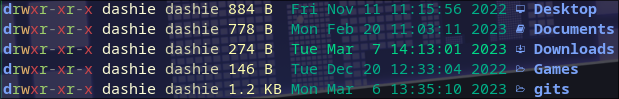
\includegraphics[scale=0.4]{2023_03_07_05_32_03.png}\newline
\textcolor{purple}{These rights are also stored as Macros in POSIX -> "sys/stat.h"}\newline
These can be chained with | -> S\_IRWXU | S\_IRGRP

\section{File API}
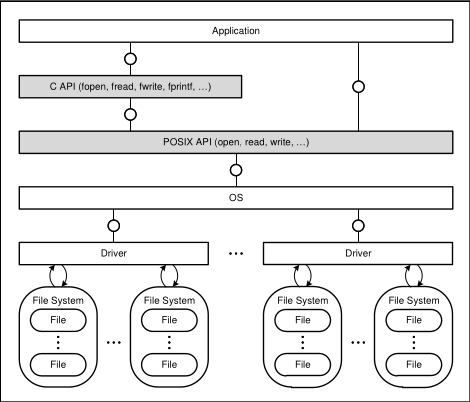
\includegraphics[scale=0.4]{2023_03_07_05_43_05.png}
\textcolor{purple}{The main difference with the POSIX API to the C API, is that the POSIX API gives us raw data, without any interpretation of the data, while the C API supports more specific things such as sockets, decoding etc.}

\subsection{POSIX File API}
General Info:
\begin{itemize}
\item \textcolor{purple}{All file functions are declared in <unistd.h> and <fcntl.h>}
\item \textcolor{purple}{error codes can be checked with "errno"}
\item \textcolor{purple}{raw data}
\item \textcolor{purple}{should only be used for binary data, not for anything that needs interpretation}
\end{itemize} 

\subsubsection{Usage of errno}
\begin{lstlisting}
if (chdir("docs") < 0) { // type is int
  if (errno == EACCESS) { // EACCESS defined in the function documentation
    printf ("Error: %s\n", strerror (errno));
    // or you can use perror
    perror ("Error"); // this makes use of the standard error stream
  }
}
\end{lstlisting}
Note, not all function set this flag, and should be used immediately, as other function will overwrite it.\newline
\textcolor{teal}{Codes for the error are directly defined in the function documentation.}\newline
\textcolor{purple}{Returns the address of a string, which describes the code in text.}\newline
perror is the same as strerror but with a special error stream.

\subsubsection{File-Descriptor}
\begin{itemize}
\item \textcolor{purple}{valid within a process}
\item \textcolor{purple}{indexed in a table of all open files in a process}
\item \textcolor{purple}{Process file table is indexed in the global table of all open files}
\item \textcolor{purple}{Receives data in order to identify physical file (correct hardware with correct driver)}
\item \textcolor{purple}{State defined: knows current offset (offset of byte that will be read next)}
\end{itemize} 
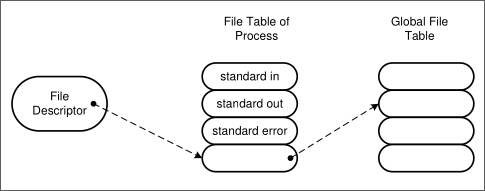
\includegraphics[scale=0.4]{2023_03_07_06_03_34.png}\newline
\textcolor{purple}{In each process open file index for a process there are 3 predefined file descriptors}\newline
\begin{lstlisting}
// STDIN_FILENO = 0  -> standard input
// STDOUT_FILENO = 1 -> standard output
// STDERR_FILENO = 2 -> standard error
\end{lstlisting}

\subsubsection{Opening files with POSIX API}
\begin{lstlisting}
int open (char *path, int flags, ...)
\end{lstlisting}
\begin{itemize}
\item \textcolor{black}{O\_RDONLY:} Read only
\item \textcolor{black}{O\_RDWR:} read and write
\item \textcolor{black}{O\_CREAT:} create file if not exists, needs another parameter for access rights
\item \textcolor{black}{O\_APPEND:} set offset to end of file before each write access
\item O\_TRUNC: set length of file to 0
\end{itemize} 

\subsubsection{Close files with POSIX API}
\begin{lstlisting}
int close(int fd)
\end{lstlisting}
deallocates file descriptor fd, which can now be used by other functions.\newline
returns 0 if ok, and -1 for error

\subsubsection{Usage of open and close}
\begin{lstlisting}
int fd = open("filename.file", O\_RDONLY);
if (fd < 0) {
  // le error handling
}
// do something with file
close(df);
\end{lstlisting}

\subsubsection{Read data with POSIX API}
\begin{lstlisting}
ssize_t read (int fd, void *buffer, size_t n)
// ssize_t is a signed size_t
\end{lstlisting}
\begin{itemize}
  \item tries to copy the next n(parameter) bytes to current offset from fd to the buffer 
\item returns count of read bytes or -1 when error
\item blocks thread until: n bytes are copied, error occurs, end of file has been reached
\item increments offset of fd by the amount of read bytes
\end{itemize} 

\subsubsection{Write data with POSIX API}
\begin{lstlisting}
ssize_t write (int fd, void *buffer, size_t n)
// ssize_t is a signed size_t
\end{lstlisting}
\begin{itemize}
  \item tries to copy the n bytes from the buffer to the offset on fd 
\item returns count of written bytes or -1 on error
\item blocks thread until n bytes are written, error occurs, or the end of file has been reached
\item increments offset of fd by the amount of bytes written
\end{itemize} 
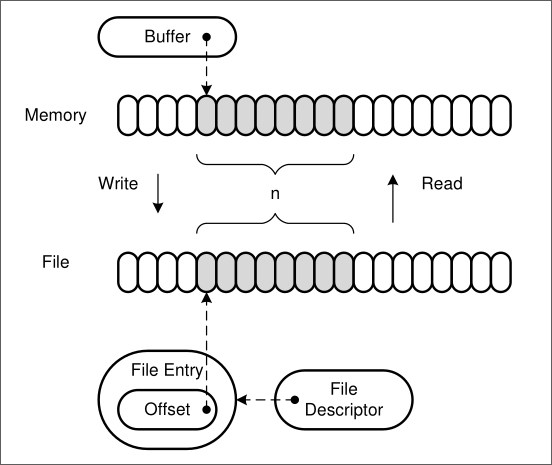
\includegraphics[scale=0.4]{2023_03_07_06_18_08.png}

\subsubsection{Jump in a file with POSIX API}
\begin{lstlisting}
off_t lseek (int fd, off_t offset, int origin)
\end{lstlisting}
\begin{itemize}
\item parameter offset that should be the new offset of fd
\item origin = SEEK\_SET for start of file
\item origin = SEEK\_CUR for current offset
\item origin = SEEK\_END for end of file
\item returns new offset or -1 on error
\end{itemize} 
Example usage:
\begin{lstlisting}
lseek (fd, 0, SEEK_CUR) return current offset
lseek (fd, 0, SEEK_END) return size of file
lseek (fd, n, SEEK_END) go beyond end of file, which will make write put 0s in this space if called. 
\end{lstlisting}
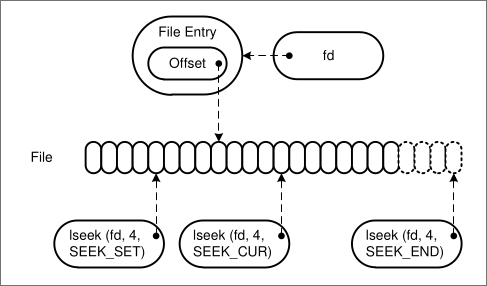
\includegraphics[scale=0.4]{2023_03_07_06_22_16.png}

\subsubsection{pread and pwrite in POSIX API}
\begin{lstlisting}
ssize_t pread (int fd, void *buffer, size_t n, off_t offset)
ssize_t pwrite (int fd, void *buffer, size_t n, off_t offset)
\end{lstlisting}
\textcolor{purple}{These are alternatives to write and read, that do not change the offset, however, this means that you will need to define where we are currently!}

\subsubsection{windoof proprietary paths}
\begin{itemize}
  \item \textbackslash instead of / because fuck you
  \item \textbackslash also needs to be escaped if you want to write it
\item root directory per disk instead of per system
\item C is the default disk, A and B were reserved for floppy disks
\item functions in windoof: \newline
  \begin{itemize}
  \item \textcolor{black}{open -> CreateFile}
  \item \textcolor{black}{read -> ReadFile}
  \item \textcolor{black}{write -> WriteFile}
  \item \textcolor{black}{lseek -> SetFilePointer}
  \item close -> CloseHandle
  \end{itemize} 
\end{itemize} 

\subsubsection{Example for reading and writing data in POSIX API}
\begin{lstlisting}
#define N 32
char buf[N];
char spath[PATH_MAX];
char dpath[PATH_MAX];

/* get paths from somewhere */

int src = open(spath, O_RDONLY);
int dst = open(dpath, O_WRONLY | O_CREAT, S_IRWXU);
ssize_t read_bytes = read(src, buf, N);
write(dst, buf, read_bytes);
close(src);
close(dst);
\end{lstlisting}

\subsection{C Stream API}
Idea: Operating systems do things differently, even something as simple as a newline is handled differently, so we need an API that can translate this to the correct symbol:\newline
\begin{lstlisting}
// Windows: \r \n = 13d 10d = 0Dh 0Ah
// Linux: \n = 10d = 0Ah
// Mac OS: \r = 13d = 0Dh (before Mac OSX, now just like penguinOS)
\end{lstlisting}
\begin{itemize}
\item \textcolor{purple}{OS independent}
\item \textcolor{purple}{stream-based: symbol-oriented}
\item \textcolor{purple}{can be buffered or unbuffered}\newline
  dependent on the implementation, transparent for applications
\item \textcolor{purple}{normally buffered for files}\newline
  independently transfers data-blocks between files and buffers
\item \textcolor{purple}{Has a file Position indicator}\newline
  - for buffered streams: defines position in buffer\newline
  - for unbuffered streams: is the offset in the file-descriptor
\end{itemize} 

\subsubsection{FILE datastructure}
\begin{itemize}
\item \textcolor{purple}{has information about a stream}
\item \textcolor{purple}{should not be used directly, instead only per pointers that are created via the C-API}
\item \textcolor{purple}{should not be copied, pointer can be used as ID by the API}
\item \textcolor{purple}{three predefined standard-streams}\newline
  \begin{itemize}
  \item \textcolor{black}{FILE *stdin}
  \item \textcolor{black}{FILE *stdout}
  \item \textcolor{black}{FILE *stderr}
  \end{itemize} 
\end{itemize} 

\subsubsection{open file with C-API}
\begin{lstlisting}
FILE * fopen (char const *path, char const *mode)
// flags
// "r": like O_RDONLY
// "w": like O_WRONLY | O_CREAT | O_TRUNC
// "a": like O_WRONLY | O_CREAT | O_APPEND
// "r+": like O_RDWR
// "w+": like O_RDWR | O_CREAT | O_TRUNC
// "a+": like O_RDWR | O_CREAT | O_APPEND
\end{lstlisting}
\begin{itemize}
\item \textcolor{black}{creates FILE-Object and stream for the file}
\item \textcolor{black}{returns pointer to created FILE-Object or 0 on error}
\end{itemize}

\subsubsection{close file with C-API}
\begin{lstlisting}
int fclose (FILE *file)
\end{lstlisting}
\begin{itemize}
\item \textcolor{black}{calls fflush}
\item \textcolor{black}{closes stream defined by file parameter}
\item \textcolor{black}{removes file from memory}
\item \textcolor{black}{returns 0 when ok, otherwise EOF}
\end{itemize} 

\subsubsection{flush of file with C-API}
\begin{lstlisting}
int fflush (FILE *file)
\end{lstlisting}
\begin{itemize}
\item \textcolor{black}{writes content to write from memory into file (if content exists)}
\item \textcolor{black}{will automatically be called when the buffer is full or file is closed}
\item \textcolor{black}{returns 0 when of, otherwise EOF}
\end{itemize} 

\subsubsection{Conversion from POSIX-API to C-API}
\begin{lstlisting}
FILE * fdopen (int fd, char const *mode)
// like fopen, but instead of path, we use a file descriptor

int fileno (FILE *stream)
// returns file-descriptor for the stream, or -1 on error
\end{lstlisting}

\subsubsection{read from file with C-API}
\begin{lstlisting}
int fgetc (FILE *stream)
\end{lstlisting}
\begin{itemize}
  \item \textcolor{black}{reads the next byte from stream \emph{as unsigned char} and returns it as int}
\item \textcolor{black}{increments the file-position indicator by 1}
\end{itemize} 
\begin{lstlisting}
char * fgets (char *buf, int n, FILE *stream)
\end{lstlisting}
\begin{itemize}
\item \textcolor{black}{reads to n-1 symbols from stream, or until newline or EOF}
\item \textcolor{black}{adds a 0 and creates a null terminated string}
\item \textcolor{black}{returns buffer(string) or 0 on error}
\item \textcolor{black}{increments the file-position indicator by the amount of read symbols}
\end{itemize} 

\subsubsection{"un"read from file with C-API}
\begin{lstlisting}
int ungetc (int c, FILE *stream)
\end{lstlisting}
\begin{itemize}
  \item \textcolor{black}{puts c(parameter -> file-descriptor) back to the stream into a special \emph{unget stack}}
\item \textcolor{black}{the next fget call will prefer the symbols in the unget stack}
\item \textcolor{black}{no change in the file itself}
\item \textcolor{black}{unget stack has a minimum size of 1 -> works at least once, can work multiple times depending on implementation}
\item returns c(parameter -> file-descriptor) or EOF on error
\end{itemize} 
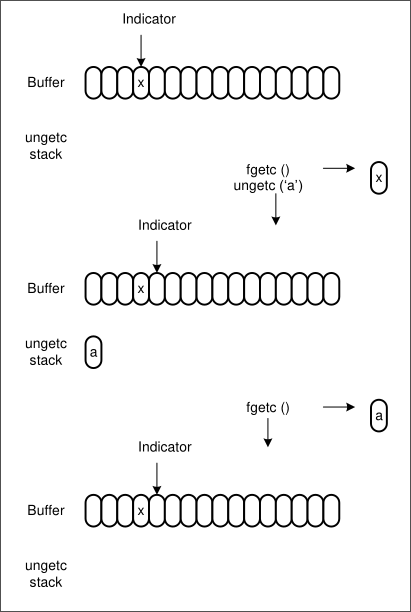
\includegraphics[scale=0.4]{2023_03_07_07_10_15.png}

\subsubsection{Write to file with C-API}
\begin{lstlisting}
int fputc(int c, FILE *stream)
\end{lstlisting}
\begin{itemize}
\item \textcolor{black}{converts file-descriptor c in unsgined char and writes it to stream}
\item \textcolor{black}{returns either c or EOF}
\item \textcolor{black}{increments the file-position indicator by 1}
\end{itemize} 
\begin{lstlisting}
int fputs (char *s, FILE *stream)
\end{lstlisting}
\begin{itemize}
\item \textcolor{black}{writes the symbols from the string s until the 0 termination symbol into the stream}
\item \textcolor{black}{the 0 termination will not be written}
\item \textcolor{black}{returns EOF on error}
\end{itemize} 

\subsubsection{End of file and Error in File C-API}
\begin{lstlisting}
int feof (FILE *stream)
// returns 0 when end of file has NOT been reached

int ferror (FILE *stream)
// retuns 0 when NO error occurred

// Example usage:
int return_value = fgetc (stream);
if (return_value == EOF) {
  if (feof (stream) != 0) {
    /* EOF reached */
  } else if (ferror (stream) != 0) {
    /* error occurred, check errno */
  }
}
\end{lstlisting}

\subsubsection{Manipulation of file-position indicator with C-API}
\begin{lstlisting}
long ftell (FILE *stream)
// returns the current file-indicator
// POSIX extension of ftello with return type off_t

int fseek (FILE *stream, long offset, int origin)
// set the file-position indicator like lseek
// POSIX extension of fseeko with off_t as type for the offset

int rewind (FILE *stream)
// reset the stream
// equivalent to fseek(stream, 0, SEEK_SET) and clear the error state
\end{lstlisting}


\subsection{Ext2}

\subsection{Ext4}

\section{Processmodels}
\subsection{Base}
Whenever we run a program, there are at least 2 actors: the program itself and the OS.\newline
The communication between OS and program runs on the C-API (or soon rust as well :) )\newline
Each program only knows itself and the OS.\newline
\textcolor{teal}{Systems like this are called \emph{monoprogramming}}

\subsubsection{Improvement with "async"}
This is what javascript does, it is only pseudo parallel in the sense that there is \emph{efficient process switching}, however we are still at 1 process at a time!\newline
There are multiple names for a process in this case -> task, job, or simply process. \newline
\newline
\textcolor{teal}{Here we still want to ensure that each program may think that is "the only running program",\newline
this means that the operating system \emph{must provide each service individually} -> memory, IO, etc. }

\subsection{Process}
\minipg{
  Each process has:
\begin{itemize}
\item \textcolor{purple}{Text section: image of the program in the memory (binary)}
\item \textcolor{purple}{data section: global variables of the program}
\item \textcolor{purple}{memory for heap}
\item \textcolor{purple}{memory for stack}
\end{itemize} 
}{
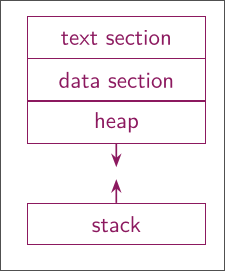
\includegraphics[scale=0.4]{2023_03_21_05_18_00.png}
}[0.25,0.25]

\subsubsection{Program vs Process}
\minipg{
Process
\begin{itemize}
\item \textcolor{purple}{active: actually executes instructions}
\item \textcolor{purple}{executes instructions in serial manner}
\item \textcolor{purple}{may perform actions for multiple programs -> according to POSIX}
\end{itemize} 
}{
Program
\begin{itemize}
\item \textcolor{purple}{passive: only says what to do}
\item \textcolor{purple}{can be run in parallel -> multiple processes execute different tasks for the program}
\end{itemize} 
}[0.25,0.25]

\subsubsection{Process Control Block (PCB)}
\textcolor{purple}{The operating system stores information about a process in this block.}
\begin{itemize}
\item \textcolor{purple}{ID for process -> PID}
\item \textcolor{purple}{Memory for the state of the processor}
\item \textcolor{purple}{scheduling information}
\item \textcolor{purple}{data for synchronization and communication between processes}
\item \textcolor{purple}{filesystem relevant information -> current open files}
\item \textcolor{purple}{Security-information}
\end{itemize} 
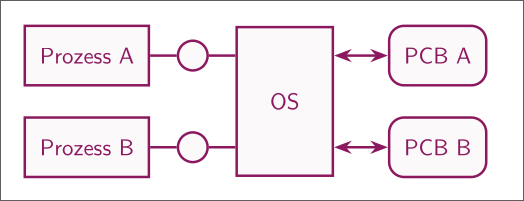
\includegraphics[scale=0.4]{2023_03_21_05_24_50.png}

\subsubsection{Interrupts, Processes and Context Switch}
\textcolor{teal}{For every interrupt the Operating system saves the current state of the process in the PCB.}\newline
The following will be saved:
\begin{itemize}
\item \textcolor{black}{Registers}
\item \textcolor{black}{Flags}
\item \textcolor{black}{Instruction Pointer}
\item \textcolor{black}{MMU-Configuration -> Page-Table-Pointer}
\end{itemize} 
\textcolor{teal}{After that, the interrupt handler will be called (which is run by the OS), which can switch context if needed -> e.g. switch to another process.\newline
As soon as the handler is done, the new context PCB is recovered.}

\subsubsection{Creation of a process}
\minipg{
POSIX:
\begin{enumerate}
\item \textcolor{purple}{create process}
\item \textcolor{purple}{load a program into this process and put it into ready mode}
\end{enumerate} 
}{
  Windoof:\newline
  both at once... (proprietary)
}[0.25,0.25]

\subsection{Process Hierarchy}
In POSIX, each process has exactly 1 parent, other than the root process.\newline
Each process can have unlimited amount of child processes!\newline
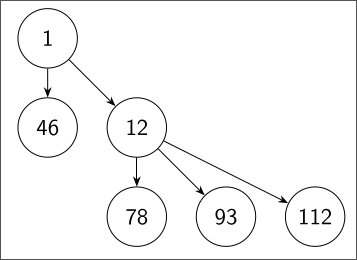
\includegraphics[scale=0.4]{2023_03_21_05_31_06.png}

\subsubsection{fork function}
The fork funcion crates an exact copy of the parent process.
\begin{lstlisting}
pid_t fork(void)
// not to mistake with :(){ :|:& };:
// kekw
\end{lstlisting}
\begin{itemize}
\item \textcolor{black}{the forked process has its own ID -> PID}
\item \textcolor{black}{the forked process has the parent ID saved as well}
\item the return of this function will be handled in \emph{both processes}\newline
  in parent: return will be either the ID or -1 for error\newline
  in child: returns 0
\end{itemize} 
Example of usage:
\begin{lstlisting}
int main() {
  pid_t new_pid = fork()
  // from here on both processes run this.

  if (new_pid > 0) {
    // this is the parent process
    // only the parent will run here
  } else if (new_pid == 0) {
    // this is the child process
    // only the child will run here
  } else {
    // error handling for parent process if forking failed
  }
}
\end{lstlisting}

\subsubsection{exit function}
\begin{lstlisting}
void exit(int code)
\end{lstlisting}
This is a return method to get out of a process.\newline
The code is simply the error handling code that you would like to pass to the parent process.

\subsubsection{wait function}
\begin{lstlisting}
pid_t wait(int* status)
\end{lstlisting}
\begin{itemize}
  \item \textcolor{black}{blocks process until \emph{one of his child processes ends}}
\item \textcolor{black}{the status will cover the return code of the child process}
\item \textcolor{black}{status usually handled with macros:}\newline
  WIFEXITED(*status) != 0 -> if child exited properly \newline
  WEXITSTATUS(*status): exit code of child
\item \textcolor{black}{will return -1 if error}\nelwine
  ECHILD: no child anymore to wait for (if false you still have children)\newline
  EINTR: was interrupted by signal
\end{itemize} 

\subsubsection{waitpid function}
\begin{lstlisting}
pid_t waitpid (pid_t pid, int *status, int options)
\end{lstlisting}
Like wait, but you can choose the child to wait for with pid.
\begin{itemize}
\item \textcolor{color}{pid > 0: waits for child with this pid}
\item \textcolor{color}{pid == -1: waits for any child -> like wait}
\item \textcolor{color}{pid == 0 and pid < -1 enables waiting for processes of a specific process group}
\end{itemize} 

\subsubsection{Examples}
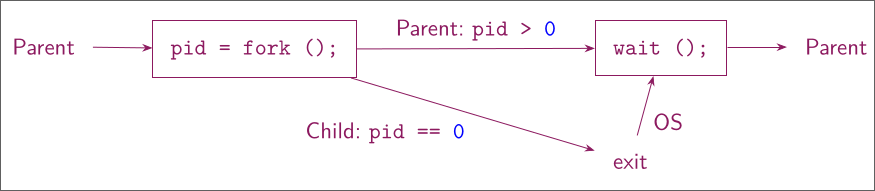
\includegraphics[scale=0.4]{2023_03_21_05_59_40.png}\newline
Worker example:
\begin{lstlisting}
#include <stdio.h>
#include <stdlib.h>
#include <sys/types.h>
#include <unistd.h>
#include <errno.h>
#include <sys/wait.h>

void spawn_worker(int a) {
  if (fork() == 0) {
    // we are in child
    printf("%d",a);
    // print number of process
    exit(0); // return code ok
  }
}

int main() {
  int pid = 0;
  for (int i = 0; i < 10; i++) {
    spawn_worker(i);
    // create 10 child processes
  }

  // do something in parent

  do {
    pid = wait(0);
    // status code is not saved!
  }

  while (pid > 0 || errno != ECHILD);
  // run until no more children!
}
\end{lstlisting}

\subsubsection{exec functions}
\textcolor{teal}{There are 6 versions of exec -> execl, execle, execlp, execv, execve, execvp}\newline
Each exec function \emph{replaces the program in the current process with another}.\newline
Parameters:
\begin{itemize}
\item \textcolor{color}{execl*: binary and args as list -> execl(path0, arg0, arg1, ...)}
\item \textcolor{color}{execv*: binary and args as vector -> execv(path, argv)}
\item \textcolor{color}{exec*e: allow array for environment variables as parameter, in the other variants the env-vars stay the same}
\item \textcolor{color}{exec*p: search for filename via environment variable PATH, the others use absolute or relative paths}
\end{itemize} 
\textcolor{teal}{the * means any character -> functions are a family}\newline
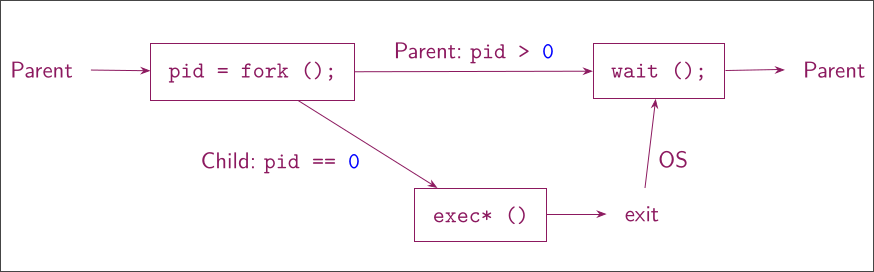
\includegraphics[scale=0.4]{2023_03_21_06_15_17.png}

\subsubsection{Zombie Processe}
\textcolor{purple}{This refers to child processes that have ended, but aren't removed yet.\newline
This means the PCB etc are all still there, but it doesn't do anything.\newline
This stays like this until the parent calls wait() for this child!}\newline
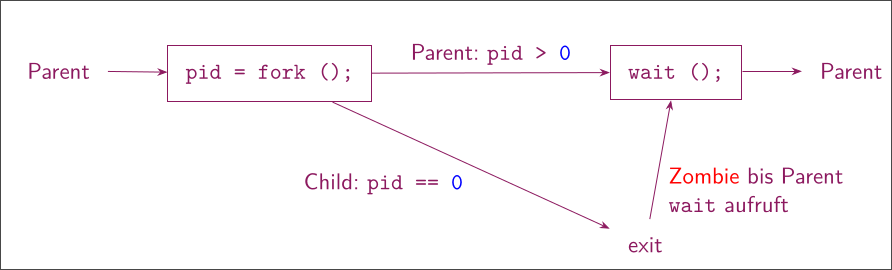
\includegraphics[scale=0.4]{2023_03_21_06_18_24.png}

\subsubsection{Orphan Process}
\textcolor{purple}{This is even worse than regular zombie processes. This means that the parent process is now dead, therefore no process can wait for this.\newline
The only solution here is an operating system process with the pid1, this process will inherit these child processes and will then continuously end all of them.}\newline
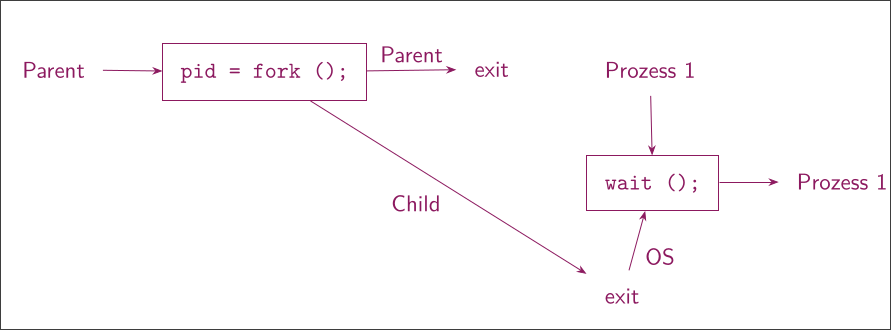
\includegraphics[scale=0.4]{2023_03_21_06_20_43.png}\newline
Note, it might be that the parent process is stuck/has an error, in this case the child processes will be passed to 1 for ending them, while the parent is killed.

\subsubsection{function sleep}
\begin{lstlisting}
unsigned int sleep(unsigned int seconds)
\end{lstlisting}
\begin{itemize}
\item \textcolor{black}{waits "closesly" for the amount of seconds provided}
\item \textcolor{black}{can be interrupted by the OS (example: signals)}
\item \textcolor{black}{returns the amount of seconds that would remain to sleep}\newline
  example if interrupted after 5 seconds, returns entered time - 5 seconds
\end{itemize} 

\subsubsection{function atexit}
\textcolor{teal}{Here you can pass functions that will be executed before the process exits.\newline
This is usefull for resources that the OS doesn't know/care about.}
\begin{lstlisting}
int atexit(void (*function)(void))
\end{lstlisting}
\begin{itemize}
\item \textcolor{black}{atexit can be called multiple times to register multiple functions}
\item \textcolor{black}{same function can be registered multiple times}
\item \textcolor{black}{functions will be called in reverse order to registered order!}
\end{itemize} 

\subsubsection{function to read pid}
These functions simply return the pid of the current process or the parent.
\begin{lstlisting}
#include <stdio.h>
#include <unistd.h>
int main() {
  pid_t my_pid = getpid();
  pid_t my_parent_pid = getppid();
  // do something with pid
}
\end{lstlisting}

\section{C Toolchain}
The toolchain handles the \emph{precompilation, compilation, assembling and linking} of executables.

\subsection{Precprocessor}
The preprocessor translates Macros and header files into actual code.\newline
The output will then be passed to the translation unit and the compiler.

\subsection{Linker}
After the individual assembly files have been assembled, the linker takes all object files and creates one executable from them.

\subsection{Loader}
\textcolor{teal}{The loader takes executables and dynamic libraries and loads them into ram.\newline
Note that static libraries are basically inside the executable.}\newline

\includegraphics[scale=0.4]{2023_03_28_05_13_22.png}

\subsubsection{Penguin Loader}
The loader under linux has the following steps: 
\begin{enumerate}
\item \textcolor{black}{exec* have syscalls on sys\_execve}
\item \textcolor{black}{searches for file, checks for permission and opens specified file}
\item \textcolor{black}{counts and copies arguments and environment variables}
\item \textcolor{black}{provides request for each registered "binary handler"}
\item Binary handler try to load data and interpret data one by one
\item program is now executed
\end{enumerate} 
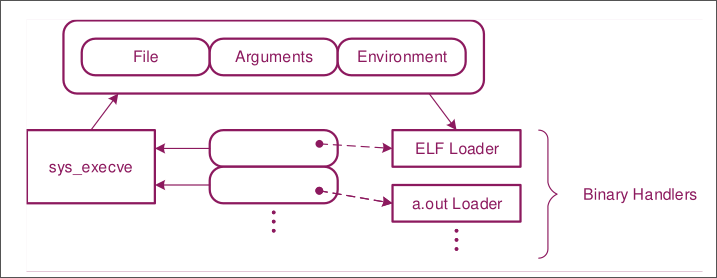
\includegraphics[scale=0.4]{2023_03_28_05_16_35.png}

\subsection{Executable Linking Format ELF}
\begin{itemize}
\item \textcolor{black}{Binary format, which specifies a program as binary}\newline
  windoof and penguin have some more than just this
\item \textcolor{black}{two possible formats}\newline
  Linking view\newline
  Execution view
\item \textcolor{black}{Used for linker and loader}\newline
  Object-File: Linking-view -> something.o
  Programs: Execution-view -> no ending?
  Shared-Objects: dynamic libraries (Linking and Execution View!) -> wlroots.so
\item \textcolor{black}{item 4}
\end{itemize} 

\subsubsection{ELF Structure}
\minipg{
\begin{itemize}
\item \textcolor{black}{Header}
\item \textcolor{black}{Program Header Table: (only necessary in execution view)}
\item \textcolor{black}{Segments: (only necessary in execution view)}
\item \textcolor{black}{Section: Header Table (only necessary in linking view)}
\item Sections: (only necessary in linking view)
\end{itemize} 
}{
\includegraphics[scale=0.4]{2023_03_28_05_20_07.png}
}[0.25,0.25]

\subsubsection{Segments and Sections}
\minipg{
\begin{itemize}
\item \textcolor{purple}{Segments and sections occupy the same memory space}\newline
  Compiler specifies space for sections\newline
  Linker specifies space for segements
\item \textcolor{purple}{Linker combines segments with the same names and defines segments}
\item \textcolor{purple}{Compiler defines sections}
\end{itemize} 
}{
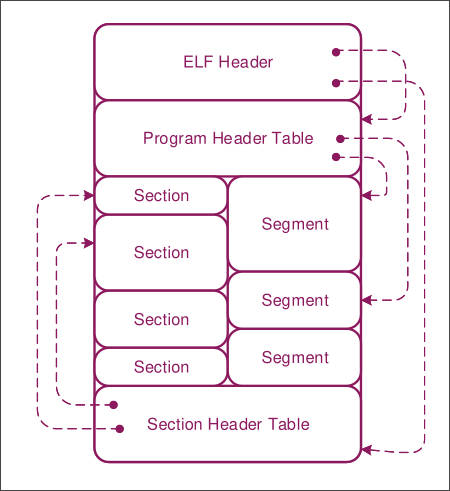
\includegraphics[scale=0.4]{2023_03_28_05_20_40.png}
}[0.25,0.25]

\subsubsection{Header of an ELF file}
\begin{itemize}
\item \textcolor{black}{52 byte: describes the structure of the file}
\item \textcolor{black}{Type: Reallocatable, executable, shared object?}
\item \textcolor{black}{32 or 64 bit}
\item \textcolor{black}{Encoding: little or big endian}
\item Machine: i386, arm, intel 64 etc
\item Entrypoint: Address at which the program should start -> main()
\item relative address, count and size of the entries for the program header table
\item relative address, count and size of the entries for the section header table
\end{itemize} 

\subsubsection{Program Header Table and Segments}
\begin{itemize}
\item \textcolor{black}{Program Header Table (or Segment Header Table): Table with n entries}
\item \textcolor{black}{Each entry is 32 bit and describes a segment}\newline
  \begin{itemize}
  \item \textcolor{black}{Segment-Type and Flags}
  \item \textcolor{black}{Offset and size of file}
  \item \textcolor{black}{Virtual address and size in memory -> possible addition: physical address}
  \end{itemize} 
\item \textcolor{black}{Segments are used at runtime by the loader}\newline
  Loader loads specified segments to memory\newline
  Loader may use more segments for other purposes: dynamic linking
\end{itemize} 
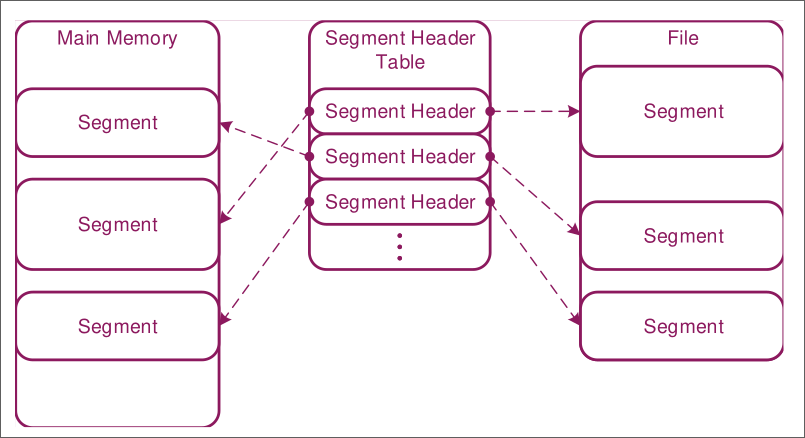
\includegraphics[scale=0.4]{2023_03_28_05_31_42.png}

\subsubsection{Sections}
\begin{itemize}
\item \textcolor{black}{Section Header Table: Table with m entries (usually :m != n | not equal sections to segments)}
\item \textcolor{black}{Each entry (40bytes) describes a section}\newline
  \begin{itemize}
  \item \textcolor{black}{Reference to string table }
  \item \textcolor{black}{Type and Flags}
  \item \textcolor{black}{Offset and Size of file}
  \item \textcolor{black}{Specific information based on section type}
  \end{itemize} 
\item \textcolor{black}{Sections will be used by linker}\newline
  \begin{itemize}
  \item \textcolor{black}{collects and concatenates(same name) sections of all object files}
  \item \textcolor{black}{generates executable}
  \end{itemize} 
\end{itemize} 
\textcolor{teal}{Section Types}
\begin{itemize}
\item \textcolor{purple}{SHT\_PROGBITS}Data defined by program, linker does not interpret this
\item \textcolor{purple}{SHT\_SYMTAB}Symbol Table
\item \textcolor{purple}{SHT\_STRTAB}String Table
\item \textcolor{purple}{SHT\_REL/RELA}Relocation Information
\item \textcolor{purple}{SHT\_HASH}Hashtable for symbols
\item \textcolor{purple}{SHT\_DYNAMIC}Information for dynamic Linking
\item \textcolor{purple}{SHT\_NOBITS}Setion without data in file
\end{itemize} 
\textcolor{teal}{Section Attributes}
\begin{itemize}
\item \textcolor{purple}{SHF\_WRITE} data of this section should be writable during execution
\item \textcolor{purple}{SHF\_ALLOC} data of this section should be in memory during execution
\item \textcolor{purple}{SHF\_EXECINSTR} data of this section display machine code
\end{itemize} 
\textcolor{teal}{Special Sections}
\begin{itemize}
  \item \textcolor{purple}{.bss:} uninitialized data
  \item \textcolor{purple}{.data:} initialized data
  \item \textcolor{purple}{.data1:} initialized data
  \item \textcolor{purple}{.debug:} debug information
\item \textcolor{purple}{rodata:} read only data
\item \textcolor{purple}{.rodata1: } read only data
\item \textcolor{purple}{.text: } executable instructions 
\item \textcolor{purple}{.symtab: } Symbol-Table 
\item \textcolor{purple}{.strtab: } String-Table 
\end{itemize} 

\subsubsetion{String Table}
\begin{itemize}
\item \textcolor{black}{Section of a file that has null terminated strings in a row}
\item Strign reference -> offset of string (starts at 0 and increases per char) 
\item \textcolor{black}{typically has names of symbols}
\item \textcolor{black}{typically does NOT include string literals like "henlo birb!", this is usually in .rodata}
\item \textcolor{black}{item 4}
\end{itemize} 
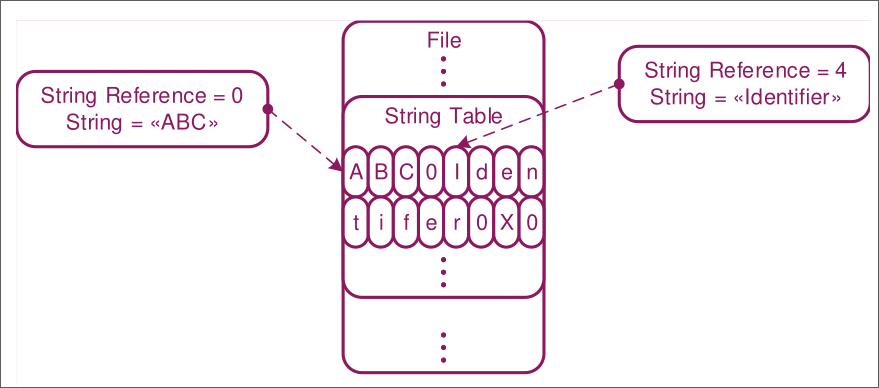
\includegraphics[scale=0.4]{2023_03_28_05_47_52.png}

\subsubsection{Symbols}
\begin{itemize}
\item \textcolor{black}{Symbol Table: each entry has 1 symbol}
\item \textcolor{black}{Symbol: 16 bytes}\newline
  \begin{itemize}
  \item \textcolor{black}{Name: 4 bytes, reference in string table}
  \item \textcolor{black}{Value: 4 bytes, depends on symbol type, could be an address for example}
  \item \textcolor{black}{Size: 4 bytes, size of symbol (for example length of function)}
  \item \textcolor{black}{Info: 4 bytes types, binding attributes (local, global, weak), reference to section header}
  \end{itemize} 
\end{itemize} 

\subsection{Static Libraries}
\begin{itemize}
\item \textcolor{black}{Static libraries are archives of object files}
\item \textcolor{black}{will be produced with the "ar" tool}
\item \textcolor{black}{named lib<something>.a -> note the ending}
\item \textcolor{black}{will only be referenced if included in compilation -> clang -lmylib}
\item static libraries are included in the binary and will receive a static address
\end{itemize} 
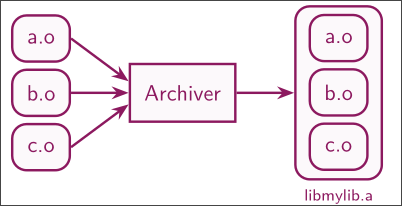
\includegraphics[scale=0.4]{2023_03_28_06_00_43.png}
\includegraphics[scale=0.4]{2023_03_28_06_00_55.png}\newline
More information:
\begin{itemize}
\item \textcolor{black}{In the early days, there were only static libraries}
\item \textcolor{green}{Will never cause a program to suddenly stop working due to updates -> it is included in binary!}
\item \textcolor{green}{easy to implement and use}
\item \textcolor{red}{Must be recompiled with program if changes are made}
\item \textcolor{red}{increases binary size}
\item \textcolor{red}{functionality can't be increased with updates to library for binaries -> again must be recompiled}
  \item \textcolor{red}{plugins impossible or only very hard}
\end{itemize} 

\subsection{Dynamic Libraries}
\begin{itemize}
\item \textcolor{black}{loaded at runtime}
\item \textcolor{red}{harder to implement}
\item \textcolor{black}{executable receives only a reference to library}
\item \textcolor{green}{library can be updated independent of binary}
\item \textcolor{red}{if binary might stop working on library updates} 
\item \textcolor{green}{Plugins are relatively easy to create}\newline
  Create API
\end{itemize} 
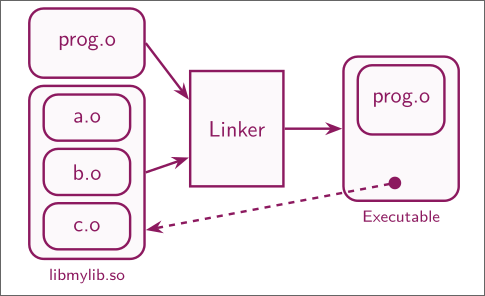
\includegraphics[scale=0.4]{2023_03_28_06_07_41.png}
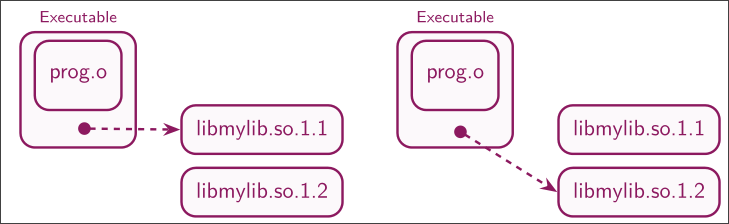
\includegraphics[scale=0.4]{2023_03_28_06_07_57.png}

\subsubsection{Delayed Loading}
\textcolor{teal}{This is essentially lazy loading for libraries, only the libraries that will be used right then and there are loaded in order to save memory.}
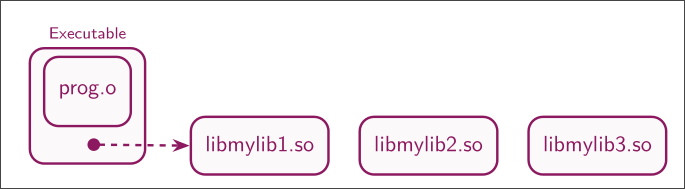
\includegraphics[scale=0.4]{2023_03_28_06_10_44.png}

\subsection{POSIX API: dynamic libraries}
\subsubsection{dlopen}
\textcolor{teal}{opens a dynamic library and returns a handle to it}
\begin{lstlisting}
void* dlopen(char* filename, int mode)
\end{lstlisting}
Mode specifies how to handle the file:
\begin{itemize}
\item \textcolor{black}{RTLD\_NOW: all symbols will be bound to the library on load}
\item \textcolor{black}{RTLD\_LAZY: symbols will be bound if needed}
\item \textcolor{black}{RTLD\_GLOBAL: } symbols can be bound used during binding of other object-files
\item \textcolor{black}{RTLD\_LOCAL: symbols can't be used for other object-files}
\end{itemize} 

\subsubsection{dlsym}
\textcolor{teal}{Returns the address of a symbol from the specified library (handle for library)}
\begin{lstlisting}
void* dlsym(void* handle, char* name)
\end{lstlisting}
\textcolor{teal}{There is no type information, you only receive an address.\newline
This means you can't know if it is a function, variable or whatever.}\newline
Example:
\begin{lstlisting}
typedef int (*func_t)(int);                // our function returns int and takes int
handle = dlopen ("libmylib.so", RTLD_NOW); // open dynamic library
func_t f = dlsym (handle, "my_function");  // take function from library and store in f
int *i = dlsym (handle, "my_int");         // take variable from library and store in i
(*f)(*i);                                  // call function
// Note we have no information about either f or i, we just assume they are function and variable respectively!
// You have to read API and documentation yourself to make sure that is the case!
\end{lstlisting}

\subsubsection{dlclose}
\textcolor{teal}{Closes the dynamic library via the specified library (handle to library)}
\begin{lstlisting}
  int dlclose(void* handle)
\end{lstlisting}
Returns 0 on success

\subsubsection{dlerror}
\textcolor{teal}{Returns a null terminated string as error if an error occurred.}
\begin{lstlisting}
  char* dlerror()
\end{lstlisting}

\subsubsection{Automatic Loading of ELF files}
As long as there is a reference to the library in the executable ELF file, libraries will automatically be loaded by need.

\subsection{Naming of Shared Objects}
\begin{itemize}
\item \textcolor{purple}{Linker-Name:} libmylib.so 
\item \textcolor{purple}{SO-Name:} libmylib.so.2
\item \textcolor{purple}{Real-Name (filename): } libmylib.so.2.1
\end{itemize} 
\textcolor{teal}{The tool "ldconfig" properly creates these files for you.}\newline
Usually only the realname exists, with the rest being \emph{soft-links}\newline
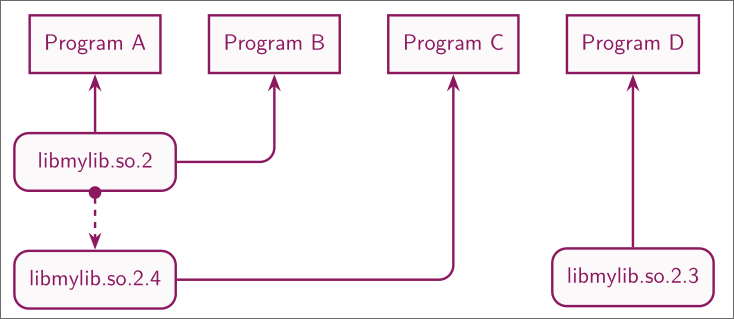
\includegraphics[scale=0.4]{2023_03_28_06_30_29.png}\newline
\textcolor{red}{As one can see, you should always use the SO name (or linker (not recommended)) at the least, if you link against the real name, then your application will break on each update...}

\subsubsection{Updates}
\begin{itemize}
\item \textcolor{black}{Real name never changes}
\item \textcolor{black}{SO-name: update on feature increases -> new API}
\item \textcolor{black}{Real-Name: update on bugfixes}
\end{itemize} 

\subsection{Shared Objects with Linker and Loader}
Linker uses the base name, the executable the SO name and the process will finally use the real name.\newline
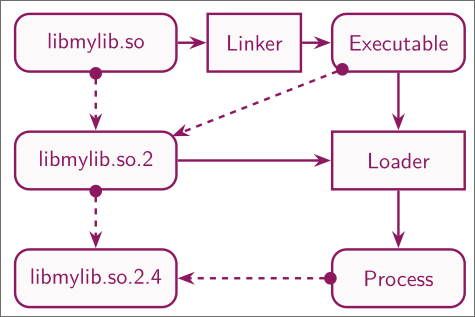
\includegraphics[scale=0.4]{2023_03_28_06_33_28.png}

\subsection{Creating Static Libraries:}
\begin{lstlisting}
// compile 
clang -c f1.c -o f1.o
clang -c f2.c -o f2.o

// create archive
ar r libmylib.a f1.o f2.o
\end{lstlisting}

\subsection{Creating Dynamic Libraries:}
\begin{lstlisting}
// compile
clang -fPIC -c f1.c -o f1.o
clang -fPIC -c f2.c -o f2.o

// create image -> .so file
clang -shared -Wl,-soname,libmylib.so.2 -o libmylib.so.2.1 f1.o f2.o -lc
\end{lstlisting}
\textcolor{red}{Important, the linker will prefer dynamic libraries, you need to override the default to use static versions if both exist}

\subsection{Using libraries}
\begin{lstlisting}
// static libraries
clang main.c -o main -L. -lmylib

// dynamic libraries
clang main.c -o main -lmylib

// dynamic library that will be called with dlopen
clang main.c -o main -ldl
\end{lstlisting}

\subsubsection{ld-linux.so effective loader}
Can be used as an executable with --list flag\newline
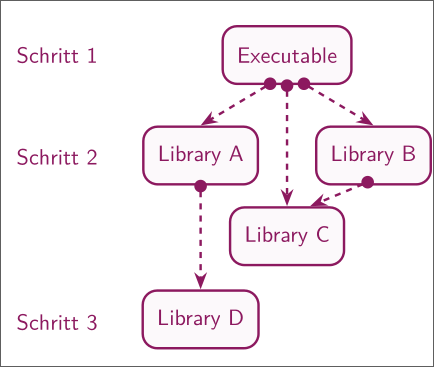
\includegraphics[scale=0.4]{2023_03_28_06_39_48.png}

\subsection{Dynamic Library Implementation}
Dynamic libraries must be able to be moved, this ofc since they are loaded into memory.\newline
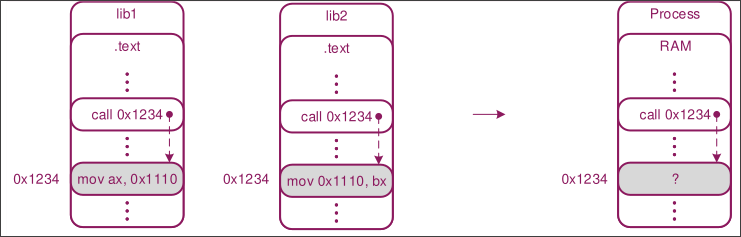
\includegraphics[scale=0.4]{2023_03_28_06_41_17.png}

\section{Communication and Synchronization}

\section{Programs and libraries}

\section{Graphical Overlays}

\end{document}
